\chapter{Tesztelés}
Ebben a fejezetben az elkészített megoldó algoritmus tesztelését mutatom be, hogy az megfelelően, hiba nélkül képes a feladatokat megoldani.
A tesztelés a következő konfigurációval rendelkező számítógéppel történt:
\begin{itemize}
	\item Processzor: Intel i5-7200, 2,50 Ghz
	\item 8 GB RAM
	\item Operációs rendszer: Windows 10
	\item Fejlesztési használt szoftverek:
		\begin{itemize}
			\item Qt Creator 4.7.1
			\item Qt 5.11.2
			\item Boost Libraries 1.68.0
			\item Microsoft Visual C++ Compiler 15.0 
		\end{itemize}		 
\end{itemize}

Az S-gráf megoldó szoftvert parancssori paraméterek segítségével lehet működtetni. A különböző megoldó módszereket, amelyek megtalálhatóak a szoftverbe implementálva, más és más kapcsolók segítéségével lehet elérni, meghívni. Ezeknek listája megtalálható a \textbf{solver} mappában lévő \textbf{README.md} fájlban. Az általam megvalósított módszerhez a következő kapcsolókat mindenképpen használni kell, hogy a program hiba nélkül fusson, végezze el az ütemezést.
\begin{itemize}
	\item \textbf{-i extended\textunderscore precedential.ods:} A bemeneti fájl elérési útvonalát kell megadni ezzel.
	\item \textbf{-o output.txt:} A kimeneti fájl elérési útvonala. Két fajta kiterjesztésű fájlt lehet megadni: \textbf{TXT} és \textbf{PNG}. Előbbi esetében a fájlba kerülnek az élek, mind a recepet, mind az ütemezési élek, valamint, hogy mennyi ideig tart a részfeladat befejezése, amelyből ezek kiindulnak. Ezenfelül a Gantt diagram karakteres formában is megjelenik. PNG kiterjesztésű fájl megadása esetén pedig kirajzolásra kerül egy Gantt diagram
	\item \textbf{-m flexbatch:} Ezzel a kapcsolóval a megoldó módszert lehet kiválasztani. A \textit{felxbatch} határozza meg, hogy az általam megvalósított algoritmus kerüljön meghívásra.
	\item \textbf{--timehor:} Időhorizont megadása történik ezzel a kapcsolóval
	\item \textbf{--obj profit\textunderscore max:} A célfüggvény kiválasztása, ebben az esetben az újonnan a megoldószoftverhez hozzáadott profit maximalizálás kerül kiválasztásra.
	\item \textbf{--precycle off:} Az precycle az ütemezés gyorsításra szolgál, mégpedig úgy, hogy előre lefut, és kört keres a gráfban. Az új módszer esetén hibásan működik, nem összeegyeztethető azzal, ezért szükséges a kikapcsolása.
	\item \textbf{--nopresolvers:} Hasonlóan az előzőhöz a presolver is az ütemezést gyorsítja, de nem egyeztethető össze az új megoldó módszerrel, emiatt kell mindenképpen inaktívvá tenni.
\end{itemize}

A ~\ref{tesztFeladat} ábrán látható mintafeladat alapján kerül bemutatásra a megoldó módszer. Két termékhez tartozó receptet látunk, illetve a részfeladatokat, valamint az ezeket megvalósítani képes berendezéseket. Az éleken megfigyelhetőek még a taszkok befejezéséhez szükséges idő.
\begin{figure}[H]
\begin{center}
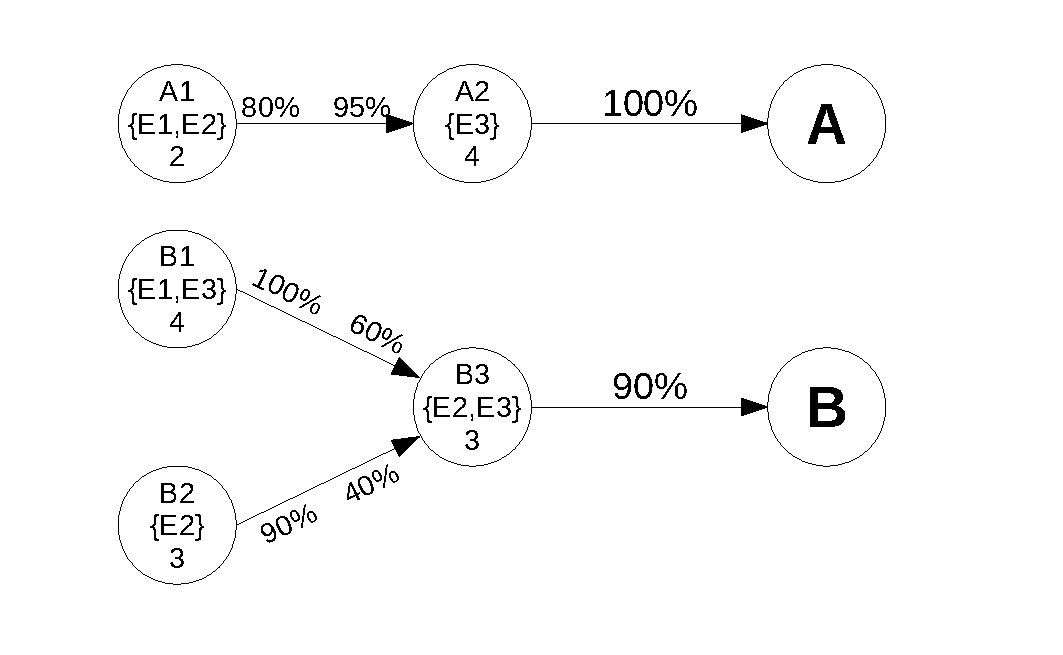
\includegraphics[scale=0.7]{tesztFeladat}
\caption{Tesztfeladat}
\label{tesztFeladat}
\end{center}
\end{figure}

\section{Taszkok közti kapacitások változtatásának hatása}
A módszer sajátossága, hogy a receptélekkel az egyes taszkok kapacitásának meghatározott százaléka hasznosítható. Ezeket a százalékokat a bemeneti fájlban lehet megadni. A példafeladat a~\ref{bemenet1} ábrán megtekinthető bemeneti adatokkal rendelkezik. Az időhorizont a bemutatott mintafeladat során 20. Látható, hogy az egyes részfeladat által lehetséges kapacitásoknak nem a teljes mennyisége kerül tovább a következő köztes feladathoz. Ez, hogy kisebb mennyiség kerül felhasználásra nagy mértékben befolyásolja a korlátot. Emellett az ütemezés megoldását is befolyásolja, mert emiatt lehetséges, hogy bizonyos berendezések nem végezhetik el az adott taszkot.

Az egyszerűség kedvéért a példában csak 2 darab A terméket és 1 darab B terméket gyártunk le. Mindkét termék legyártásából származó jövedelem mindössze egy egység. A \textit{precendce} táblában látható, hogy a taszkok által elérhető mennyiségek nem 100 százalékban kerülnek további felhasználása. Például az A1 és A2 taszkok esetében, az A1-es taszk mennyiségének 80 százaléka kerül továbbítása, illetve ennek a már kisebb mennyiségnek a 70 százalékát veszi fel az A2-es részfeladat. A \textit{proctime} táblán megtalálhatjuk, hogy melyik taszkot, melyik berendezés tudja elvégezni, valamint ezt mennyi idő alatt.
 
\begin{figure}[H]
\begin{center}
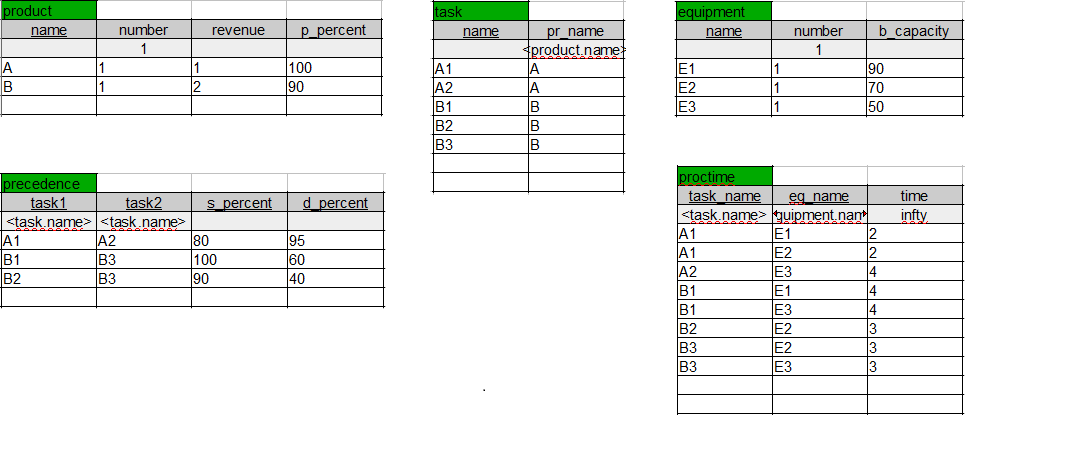
\includegraphics[scale=0.7]{bemenet1}
\caption{Első feladat bemeneti adatai}
\label{bemenet1}
\end{center}
\end{figure}

A feladat megoldását tartalmazó TXT kiterjesztésű fájlt három darab elkülöníthető részre tudjuk felosztani. Az első része látható a~\ref{eredmeny1} ábrán. Az ábra elején az éleket találhatjuk meg, mégpedig olyan formában, hogy melyik taszkból melyik taszkba mutat. Továbbá láthatók idő értékek, amelyek megadják, hogy az élt megelőző részfeladatot mennyi idő alatt lehet elvégezni. Ez a rész tartalmazza mind a receptéleket, mind az ütemezési éleket. Úgy tudjuk ezeket elkülöníteni, hogy amelyikhez 0 időérték van rendelve, azok tartoznak a az ütemezési élek csoportjához. Mivel az egyik termékből, nevezetesen az A-ból, több mint egy darabot gyártunk ezért megkülönböztetjük az egyes receptekhez tartozó feladatokat. Láthatunk A1-et és A1\textunderscore 2-t. Ugyanolyan típusú feladatról beszélünk, de különböző recepthez tartoznak, ezért kell megkülönböztetni egymástól ezeket. 
\begin{figure}[H]
\begin{center}
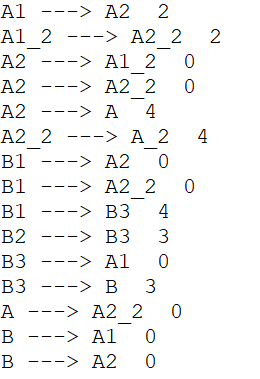
\includegraphics[scale=0.8]{eredmeny1}
\caption{A megoldást tartalmazó fájl első része}
\label{eredmeny1}
\end{center}
\end{figure}
A második részben a taszkok és a hozzájuk tartozó kapacitások, valamint a termékekhez tartozó kapacitások és a termékek előállításából származó jövedelem szorzata található. Ezeket követően szerepel a bound, a korlát, ami az adott feltételek és adatok mellett 173,846 lett. Ezt úgy kapjuk meg, hogy a termékekhez tartozó értékeket összeadjuk. Jelen példa esetében 3 érték kerül összeadásra, ezek a következők: A2, A2\textunderscore 2, és a B3. Az A2-es és a A2\textunderscore 2-es részfeladatok kapacitása 60, a B3-as taszk kapacitása pedig 53,846. Mivel a példában mindkét termék esetében a jövedelem egy, ezért az érték marad változatlanul a termékeknél. Ezeket összeadva kijön a 173,846, ami megegyezik a szoftver által kiszámolt megoldással. Ezek az értékek a~\ref{eredmeny2} ábrán megtekinthetőek.
\begin{figure}[H]
\begin{center}
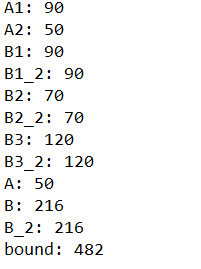
\includegraphics[scale=0.85]{eredmeny2}
\caption{A megoldást tartalmazó fájl második része}
\label{eredmeny2}
\end{center}
\end{figure}
Az utolsó szakaszban a Gantt diagram karakteres formában található meg. Látható, hogy a megadott bemeneti adatok alapján minden lehetséges taszk és berendezés kombináció elő áll. A\ref{eredmeny3} ábrán látható ez. 
\begin{figure}[H]
\begin{center}
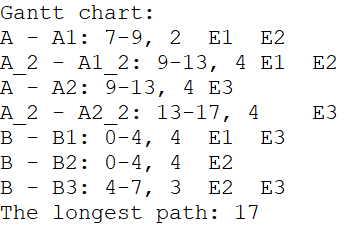
\includegraphics[scale=0.85]{eredmeny3}
\caption{A megoldást tartalmazó fájl második része}
\label{eredmeny3}
\end{center}
\end{figure}
A következő esetben újra lefuttatjuk a példafeladatot, azzal a kis változtatással a bemeneti adatokon, hogy az élekhez tartozó százalékok mindegyikét felemeljük 100 százalékra, vagyis a teljes mennyiség minden taszk esetében tovább kerül a következő részfeladathoz. A többi adat, köztük a kapcsolóval megadott idő horizont is változatlan marad. 

Ahogy várható volt az újbóli futtatás során eltérések vannak az előzőhöz képest. Egyik legfontosabb eltérése, hogy a bound megváltozott. Ebben az esetben már csak 170 lett. A jelenlegi futás során a bound kereken 170 lesz. További eltérése, hogy most már nem minden lehetséges taszk - berendezés pár lett összerendelve, mert abban az esetben a megadott idő horizonton belül nem lenne megoldható a feladat. A változás a B3-as taszk esetében történt meg. Az E3-as berendezés már nem lett hozzárendelve, azaz ezt a feladatot nem végzi el. A megoldó szoftver által elkészített png kiterjesztésű fájl látható a~\ref{output2} ábrán. Könnyen leolvasható, hogy a berendezések párhuzamosan képesek ugyanazt a taszkot elvégezni. Erre példa a B1-es köztes feladat rögtön az ütemezés elején. 

\begin{figure}[H]
\begin{center}
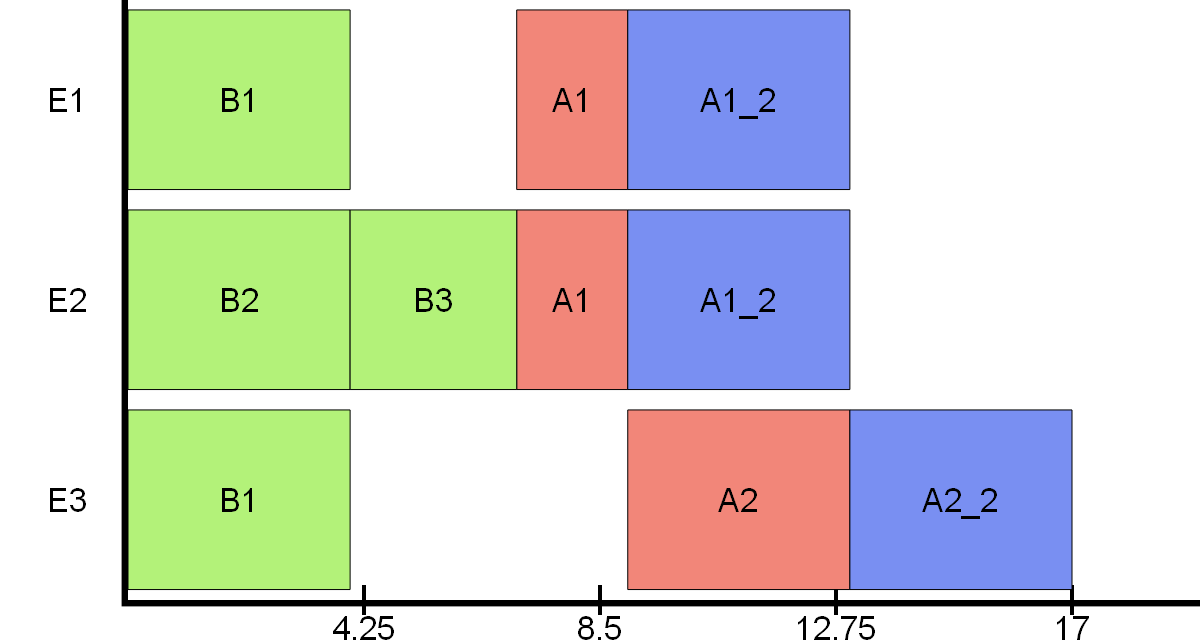
\includegraphics[scale=0.5]{output2}
\caption{A solver által elkészített Gantt diagram}
\label{output2}
\end{center}
\end{figure}

\section{Idő horizont változtatás}
A parancssori paraméterben megadott idő horizont is fontos szerepet tölt be az ütemezés során. Az eddig bemutatott példáknál nem változott meg. Ebben a részben viszont ennek a változtatására bekövetkező változások bemutatása a cél. Az idő horizont azt az időt adja meg, amelyen belül meg kell oldani a feladatot.

Minden receptnek van egy olyan minimális ideje, amely alatt nem teljesíthető. Ha ennél kisebbet adunk meg, akkor a feladat megoldhatatlan, elvégezhetetlen lesz. A \ref{tesztFeladat} ábrán látható feladat esetében, amelyet a~\ref{bemenet1} táblákban szereplő adatokkal futtatunk, ez a mindenképpen szükséges idő 12 egység lesz. Szóval ha 11 vagy annál kisebb idő horizontot adunk meg, akkor nem kapunk megoldást a feladatra. A Minden egyes gyártási munkafolyamat során találunk egy felső határt, amelynél hiába biztosunk több időt a munkafolyamat befejezésére, nem lehet nagyobb bevételre szert tenni. A mintafeladatnál ez 17 időegységnél következik be. Ebben az esetben minden berendezés elvégzi azokat a taszkokat, amelyeket el is tud végezni. A példából láthatjuk, hogy minél több idő van a feladat megoldására, annál nagyobb bevételre tehetünk szert. Ennek oka az, hogy több berendezést tudunk beállítani adott feladat elvégzésére, mert már belefér abba az időtartamba, amelyet korlátként megadtunk. Láthatjuk a 15 és 16 időegység esetében, hogy hiába biztosítunk nagyobb idő horizontot nem tudunk nagyobb bevételt elérni. Ilyen eset akkor fordulhat elő, mikor egy részfeladat elvégzéséhez szükséges idő nagyobb, mint amekkora szabadon fennmaradó idővel rendelkezünk még a határ alatt.  

\begin{table}[H]
	\begin{center}
		\caption{Adott időhorizont alatt elérhető bevételek}
  		\captionsetup[table]{skip=10pt}
    	\label{tab:table2}
		\begin{tabular}{|c|c|c|c|c|c|c|c|}
		\hline
		Idő horizont & \textless =11 & 12 & 13 & 14 & 15,16 & \textgreater =17\\
		\hline
		Max bevétel & nem megoldható & 139,048 & 153,333 & 155,714 & 159,56 & 173,846\\
		\hline
		\end{tabular}	
	\end{center}	
\end{table}

\section{Második tesztfeladat}
A második tesztfeladat során két fajta terméket kell gyártani. Az A termék előállításához 2 részfeladatot kell elvégezni, a B termék esetében pedig 2 darabot. Ehhez 2 darab berendezés áll rendelkezésre, az E1 és E2 elnevezésű berendezés. A\ref{tesztFeladat2} ábráról leolvasható, hogy melyik taszkot melyik berendezés képes elvégezni. A1-es taszkot mindkét berendezés, A2-es taszkot csak az E1, A3-as taszkot pedig csak az E2-es berendezés tudja végrehajtani. A másik termék esetében mindkét taszkot mindkét berendezés képes megvalósítani.

\begin{figure}[H]
\begin{center}
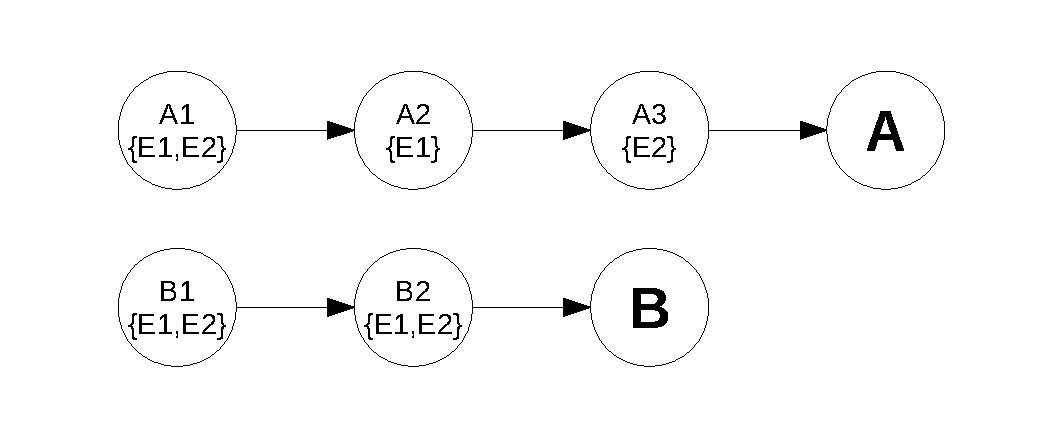
\includegraphics[scale=0.7]{tesztFeladat2}
\caption{Második tesztfeladat}
\label{tesztFeladat2}
\end{center}
\end{figure}

A \ref{tab:table3} táblázatban láthatóak a mintafeladaton elvégzett tesztesetek kiemelt adatainak első része. Továbbiak megtalálhatóak a függelékben. A teszteléssel kapcsolatos fájlok a CD melléklet \textbf{Teszteles} mappában vannak. Ezen belül a bemeneti adatokat tartalmazó fájlok fellelhetőek a \textbf{Input\_fajlok} mappában. A megoldást megjelenítő Gantt diagramot pedig a \textbf{Megoldasok} mappában tekinthetőek meg.

\begin{table}[H]
	\begin{center}
	\caption{Második példafeladat tesztesetei}
  	\captionsetup[table]{skip=10pt}
  	\label{tab:table3}
  	\begin{sideways}
  		\begin{tabular}{|c|c|c|c|c|c|c|c|c|}
  		\hline
		Fájl név & Idő horizont & A termék & B termék & Kapacitások & Hozzárendelések & Bevétel & Megoldás ideje & Gantt \\
		\hline
		teszt01 & 13 & 1 db & 1 db & \makecell{A1: 60\\A2: 40\\A3: 40\\B1: 60\\B2: 60} & \makecell{E1: A2\\ E2: A1, A3,\\ B1, B2} & 700 & 0,059 sec & er01 \\
		\hline
		teszt02 & 15 & 1 db & 1 db & \makecell{A1: 100\\A2: 40\\A3: 40\\B1: 100\\B2: 100} & \makecell{E1: A1, A2\\B1, B2\\ E2: A1, A3,\\ B1, B2} & 900 & 0,029 sec & er02 \\
		\hline
		teszt03 & 13 & 1 db & 1 db & \makecell{A1: 60\\A2: 40\\A3: 40\\B1: 60\\B2: 60} & \makecell{E1: A2\\ E2: A1, A3,\\ B1, B2} & 700 & 0,060 sec & er03 \\
		\hline
		teszt04 & 15 & 1 db & 1 db & \makecell{A1: 100\\A2: 40\\A3: 40\\B1: 100\\B2: 100} & \makecell{E1: A1, A2\\B1, B2\\ E2: A1, A3,\\ B1, B2} & 900 & 0,028 sec & er04 \\
		\hline
		teszt05 & 20 & 2 db & 1 db & \makecell{A1: 60\\A1\_2: 100\\A2: 40\\A2\_2: 40\\A3: 40\\A3\_2:40\\B1: 60\\B2: 60} & \makecell{E1: A1\_2, A2,\\A2\_2 \\ E2: A1, A1\_2,\\ A3, A3\_2, \\ B1, B2} & 1100 & 0,084 sec & er05 \\
		\hline
		\end{tabular}
	\end{sideways}
	\end{center}
\end{table}

Első oszlopban a bemeneti adatokat tartalmazó fájl neve szerepel. Ennek kiterjesztése minden esetben \textit{ods}. Másodikban az időhorizont szerepel, amelyet parancssori paraméterben kap meg a megoldó szoftver. Harmadik és negyedik oszlopban az egyik, illetve másik termékből legyártott mennyiség szerepel. Ötödik oszlopban az egyes taszkok kapacitása van. A hatodikban kapnak helyet a taszk és berendezések közötti hozzárendelések. Hetedik oszlopban a termelés során elért bevétel értéke látható. Utolsó előtti oszlopban az az idő szerepel, ameddig a szoftver végezte az ütemezést. Végezetül az utolsó oszlopban a Gantt diagramot tartalmazó fájl neve szerepel, aminek kiterjesztése \textit{png}.

A teszteknél ugyanazon feladat különböző bemeneti adatokkal került tesztelésre. Minden esetben változatlan marad a termékek elkészítéséből származó jövedelem. Ez az A termék esetén 10 egység, B termék esetében pedig 5. A berendezések kapacitása, amely alapján a taszkok kapacitása alakul, szintén állandó marad a tesztesetekben. Az E1-es berendezés kapacitása 40, az E2-es berendezésé pedig 60. Ezeken kívül az sem változik, hogy az adott taszkokat mennyi ideig tart elvégezni. Ezek az adatok megtekinthetőek a tesztek bementi fájljaiban.

Az első 4 teszt során mindegyik termékből 1 darabot gyártunk. Első esetben 13-nak adtam meg az időhorizontot, így a bevétel 700 lett. A második tesztnél ezt az értéket megnöveltem 15-re, így 900 egységre emelkedett a bevétel. Ez annak köszönhető, hogy az E1-es berendezés az első esetben csak 1 taszk elvégzésért felelős. A második esetben viszont még 3 darab taszkot elvégez a párhuzamosan végezhető munka engedélyezésre révén, így ezeknek a  taszkoknak a kapacitása megnövekedett és nagyobb mennyiséget áll elő. E két tesztnél a kapacitások 100 százaléka fel van használva. Ebben tér el a harmadik és negyedik teszt. Ott ugyan 50 százalékra van ez csökkentve, de az arány ugyan akkora lesz, így a végső kapacitások, melyekből a jövedelem származik, sem változnak, így maradnak az eddigi elérhető legjobb bevételek. Későbbi teszteseteknél majd előjön, hogy miként változik az ütemezés ennek hatására.

Az ötödik, hatodik, hetedik és nyolcadik tesztesetben 2 darab A termék és 1 darab B termék kerül legyártásra. Az ötödik tesztnél az időhorizont 20 és a kapacitások teljes mennyiségben felhasználásra kerülnek. Így a bevétel 1100 egység lesz. Miután az idő horizontot megemeltem a bevétel megnőtt 200 egységgel, így 1300 lett. Ez abból következik, hogy az E1-es berendezés az E2-es berendezéssel egyetemben már az A1, B1, B2-es taszkokat is elvégzi. A hetedik és nyolcadik tesztnél észrevehető, hogy lecsökken a bevétel. Ez a korábban említett kapacitások mennyiségének továbbvitelének megváltozásából következik. Az A1-es és A2-es közötti élen lévő arány 2 az 1-hez, míg az A2 és A3 között 1 a 2-höz. Az előző fejezetekben említett képlet, ahol a kapacitást szorozzuk ezzel az aránnyal, adja meg, hogy kevesebb lesz az A3as taszk kapacitása. Mivel 2 darab A termék kerül legyártásra, így duplán számolódik ez a bevételnél. 

Ez számokban kifejezve:
\begin{itemize}
	\item[] A1 kapacitása 100
	\item[] A2 kapacitása a következő számításból adódik: $100*(100/50)$ Ez 200 lesz, de mivel ez nagyobb, mint az berendezésből adódó kapacitás, ezért nem ez fog számítani. Mivel ezt a taszkot az E1-es berendezés végzi el, aminek 40 lesz a kapacitása, így a tényleges kapacitása az A2-es taszknak is 40 lesz.
	\item[] Az előző számításhoz hasonlóan kapható meg az A3-as taszk kapacitása. A3-as berendezéséből adódó kapacitás szorozva az éleken szállított  kapacitás arányával. Számokban ez a következő: $40*(50/100)$ Ez 20 lesz, ami a legkisebb a korlátok közül, így ezt kapja meg a taszk.
	\item[] A termékből származó jövedelem 10. 20 egység van 1 darab A termék esetén, ezt megszorozzuk az említett jövedelemmel kijön a 200. 2 darab A terméket gyártunk le, ezért összesen az A gyártásból származó jövedelem 400 lesz.
	\item[] B termék esetében nem vezetem le, hogyan jön ki az 500as bevétel, mert megegyezik az A termék esetén bemutatott levezetéssel.
	\item[] A két fajta termékből származó bevételt összeadva megkapjuk a 900 egységnyi összbevételt.
\end{itemize}
